% ju 28-Nov-24 mein-dokument.tex
\documentclass{vorlage-design-main}
% Verwenden von fontspec und unicode-math für XeLaTeX oder LuaLaTeX

%% Ganze Überschrift
\title{Anwendung von Markdown-Techniken für Dokumentationen}
%% Kürzerer Titel
\runningtitle{Dokumentation mit Markdown}
\author{Jan Unger}
\date{\today}

%% Referenzen
\addbibresource{literatur.bib}

\begin{document}

\maketitle

\begin{abstract}
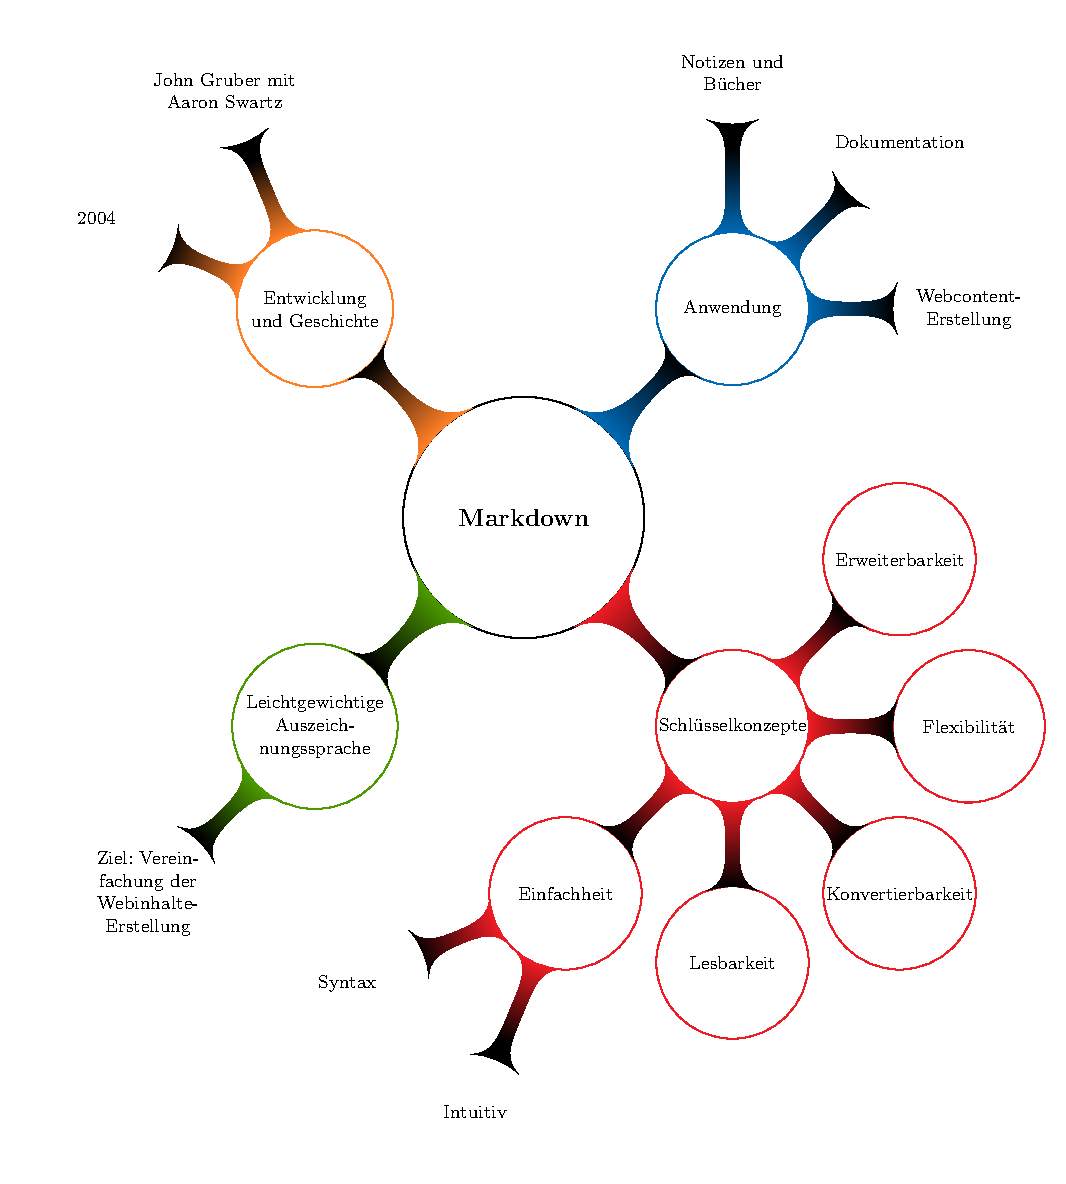
\includegraphics[width=0.5\textwidth]{images/Mindmap-Markdown.pdf}

Markdown ist eine leichtgewichtige Auszeichnungssprache, die entwickelt
wurde, um das Schreiben von Webinhalten zu vereinfachen. Sie ermöglicht
es Autoren, mit einer einfachen Textformatierungssyntax Dokumente zu
erstellen, die dann in HTML umgewandelt werden können. Markdown wurde
2004 von John Gruber in Zusammenarbeit mit Aaron Swartz entworfen, mit
dem Ziel, Lesbarkeit und Einfachheit in den Vordergrund zu stellen.

Git ist ein weit verbreitetes Versionskontrollsystem, das von
Entwicklern verwendet wird, um den Überblick über Änderungen an ihren
Codeprojekten zu behalten. Es unterstützt die Zusammenarbeit, indem es
mehreren Benutzern ermöglicht, an denselben Projekten zu arbeiten, ohne
sich gegenseitig zu behindern.

Python ist eine weit verbreitete, hochgradig vielseitige
Programmiersprache, die für ihre Einfachheit und Lesbarkeit bekannt ist.
Sie unterstützt verschiedene Programmierparadigmen wie objektorientiert,
imperativ und in gewissem Maße auch funktional.

\textbf{Keywords:} Markdown, Pandoc, Konvertierung
\end{abstract}

\section{Dokumente in Markdown
erstellen}\label{dokumente-in-markdown-erstellen}

\begin{lstlisting}
// Projektübersicht
Entwicklung               git_hilfsprogramm.py      mein-dokument.fls
LICENSE                   html                      mein-dokument.tex
Makefile                  image_resizer.py          navigation.css
NAVIGATION.html           images                    python-scripte
README.md                 literatur-kfz.bib         scriptauswahl.py
TODO.md                   literatur-sport.bib       tex
Tabellen                  literatur.bib             vorlage-design-main.cls
content                   md
dokumentation.py
\end{lstlisting}

Git

\begin{figure}
\centering
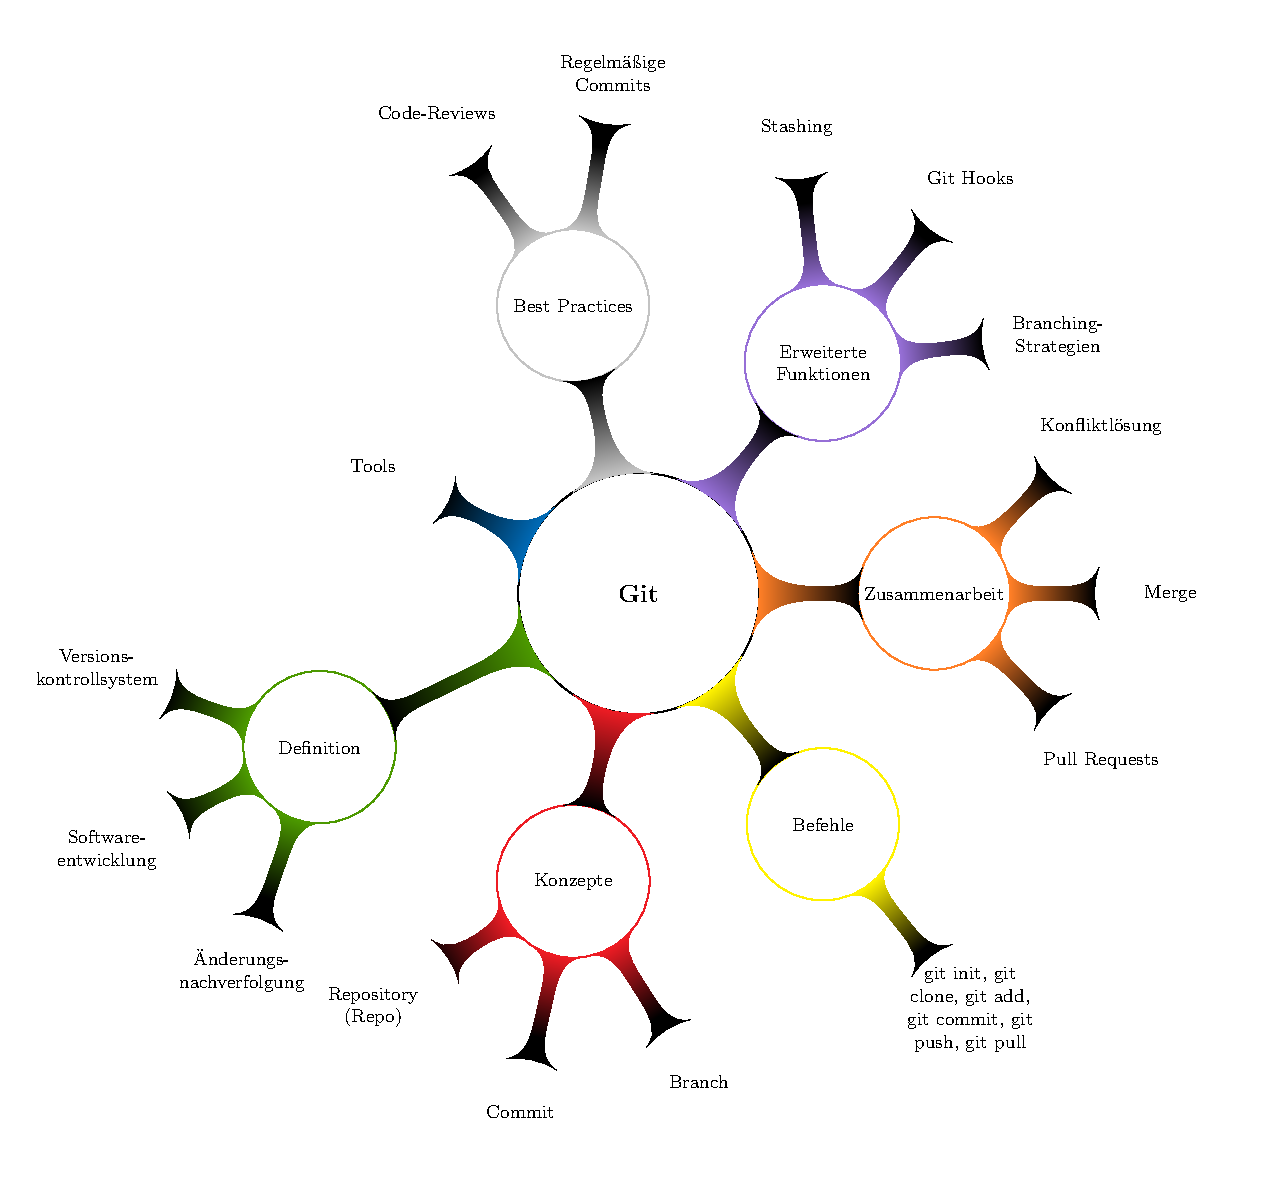
\includegraphics[width=0.6\linewidth,keepaspectratio]{images/Mindmap-Git.pdf}
%\floatnotes{}
%\label{fig:}
\caption{Was ist Git?}
\end{figure}

\begin{lstlisting}[language=bash]
# Git Versionierung
gh auth login
git config --global credential.helper cache

git remote -v

git init --bare
git remote add local /Users/jan/notizen_latex_html_python_v1.git
git remote rename localBackup local
git push local main
git pull local main

git init
git remote set-url origin https://github.com/ju1-eu/notizen_latex_html_python_v1.git
git push -u origin main
git pull origin main

git push
git pull
git  st
git ls

git clone https://github.com/ju1-eu/notizen_latex_html_python_v1.git
git clone /Users/jan/notizen_latex_html_python_v1.git notizen_klon
\end{lstlisting}

Latex

\begin{lstlisting}[language=bash]
wget https://mirror.ctan.org/systems/texlive/tlnet/update-tlmgr-latest.sh
sudo sh update-tlmgr-latest.sh -- --accept

sudo chown -R $(whoami) /usr/local/texlive/

# Pakete installieren
tlmgr install pgf

# alle installierten Pakete zu aktualisieren
tlmgr update --all

# Überprüfung der Installation
tlmgr --version
tlmgr list --installed
\end{lstlisting}

Beispiel Quellenangabe

\begin{itemize}

\item
  Fachbuchautor \textcite{dalwigk:2024:fachbuchautor}.
\item
  Online Kurse \textcite{schaffranek:2024:kurse}.
\item
  Hacking und Cyber Security mit KI \textcite{dalwigk:2023:hacking}.
\item
  Python für Einsteiger \textcite{dalwigk:2022:python}.
\item
  Mikrocontroller ESP32 \textcite{brandes:2023:mikrocontroller}.
\item
  Roboterauto \textcite{brandes:2022:esp32}.
\item
  Daten mit Raspberry Pi im Netz speichern und visualisieren
  \textcite{brandes:2023:daten}.
\end{itemize}

Hier ist ein Text, der eine Fußnote benötigt.\footnote{Text der Fußnote.}

Liste

\begin{enumerate}
\def\labelenumi{\arabic{enumi}.}

\item
  eins
\item
  zwei
\end{enumerate}

\textbf{Tabelle 1:} Diese Tabelle gibt eine übersichtliche Darstellung
der ausgeführten Skripte, ihrer jeweiligen Funktionen und der Ergebnisse
der Ausführung.

\begin{table}[ht]
  %\caption{}
  %\label{tab:my-table}
  \begin{tabular}{@{}lll@{}}
\toprule
Skriptname
 &
Beschreibung
 &
Ergebnis
 \\
\midrule[\heavyrulewidth]
\verb|html\_konverter\_pandoc1.py| & Konvertiert
HTML-Dokumente mit Pandoc & Erfolgreich abgeschlossen \\
\verb|html\_dateien\_verarbeiten2.py| & Verarbeitet
HTML-Dateien & Erfolgreich abgeschlossen \\
\verb|navigationsseite\_html.py| & Erzeugt
Navigationsseiten mit Jinja2 & Fehler: Modul `jinja2' nicht gefunden \\
\verb|html\_entfernen2.py| & Bearbeitet die Datei
mein-dokument.html & Erfolgreich abgeschlossen \\
\bottomrule
\end{tabular}%
\end{table}

\newpage

\begin{lstlisting}[language={C++}]
// Quellcode: HalloWelt.cpp
#include <iostream>

int main() {
    std::cout << "Hallo Welt" << std::endl;
    return 0;
}
\end{lstlisting}

\begin{lstlisting}
// Markdown
[Google](https://www.google.com)

![Logo 2](images/Logo/Logo2.pdf){width=50%}
\end{lstlisting}

Website \href{https://www.google.com}{Google} und GitHub
\url{https://github.com/ju1-eu} und meine Website
\url{https://bw-ju.de/}

\begin{figure}
\centering

\includegraphics[width=0.4\linewidth,keepaspectratio]{images/Logo/Logo2.pdf}
%\floatnotes{}
%\label{fig:}
\caption{Logo 2}
\end{figure}

\begin{figure}
\centering
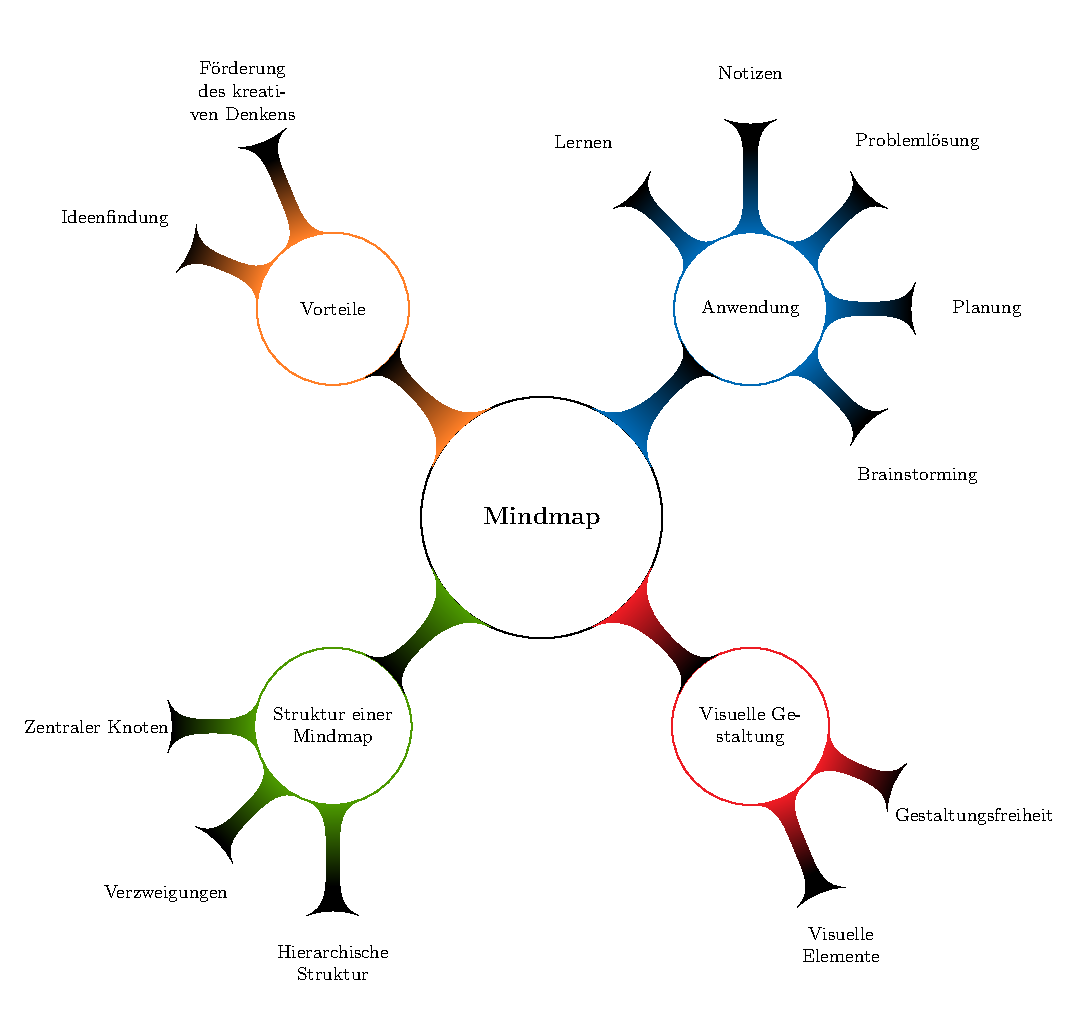
\includegraphics[width=0.6\linewidth,keepaspectratio]{images/Mindmap.pdf}
%\floatnotes{}
%\label{fig:}
\caption{Was ist eine Mindmap?}
\end{figure}

\begin{figure}
\centering
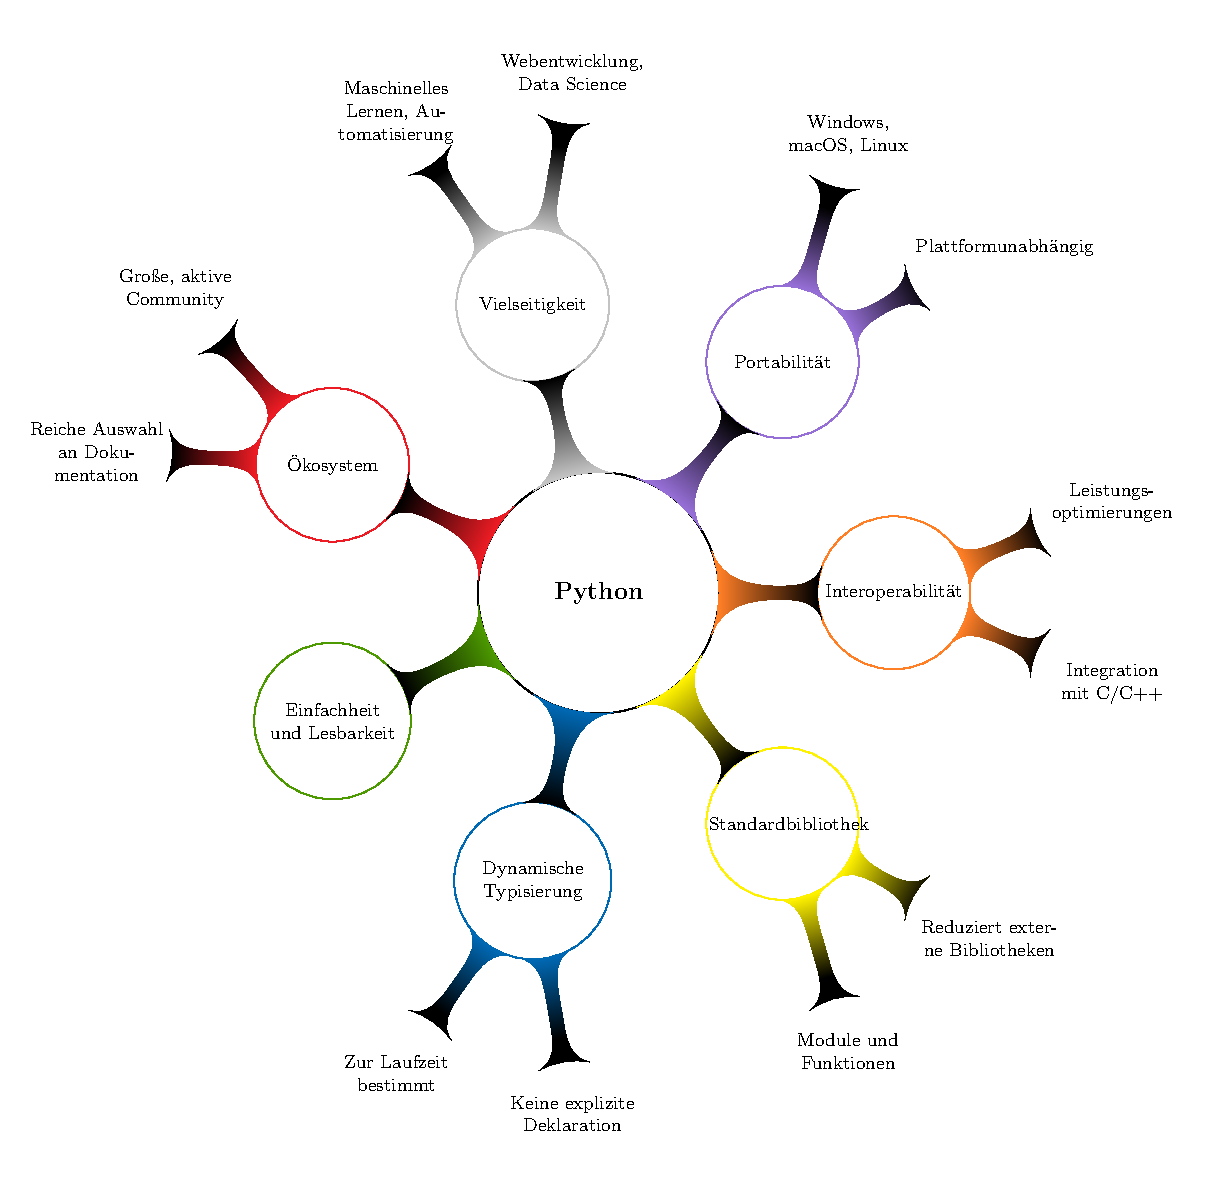
\includegraphics[width=0.6\linewidth,keepaspectratio]{images/Mindmap-Python.pdf}
%\floatnotes{}
%\label{fig:}
\caption{Was ist Python?}
\end{figure}

%% Anhang
%\clearpage
%\appendix

\clearpage
\printbibliography
\end{document}
